\section{Application Structure}

The structure of \projectname{} is a bit different from other web applications.

\subsection{Architecture}

The architecture of \projectname{} differs from other web applications in the way that there exists two different type of servers. 
The architecture can be seen in figure~\ref{fig:system_architecture}
The server where the web application is running is called Master denoted M.
For each drone in the system there is a Slave denoted S. 
On both M and S there exists daemons which is responsible for different tasks, however there is some similarity that is that these tasks can happen at anytime therefore the program needs to be running at anytime. These daemons are denoted D.
Each user have a browser they view the application through this is denoted B.
It is M's responsibility to communicate with every S in the system.
S is responsible for all communication with the drone it is parred with.

When a user wants to interact with a drone it will be with a session key. Such a session key is generated by S and then given to B through M. When both B and S have the same session key it is possible for them to communicate without M. This was done to remove the possibility of M becoming a bottleneck and to reduce latency of the interaction.

The architecture is scalable because when a new drone is added it is controlled by its S. This was done so the system could scaled out and not up. Scale out means using a lot of small machines where scale up means adding more processors, ram etc. to the server so it can handle more by itself.

\begin{figure}[htb]
    \centering 
    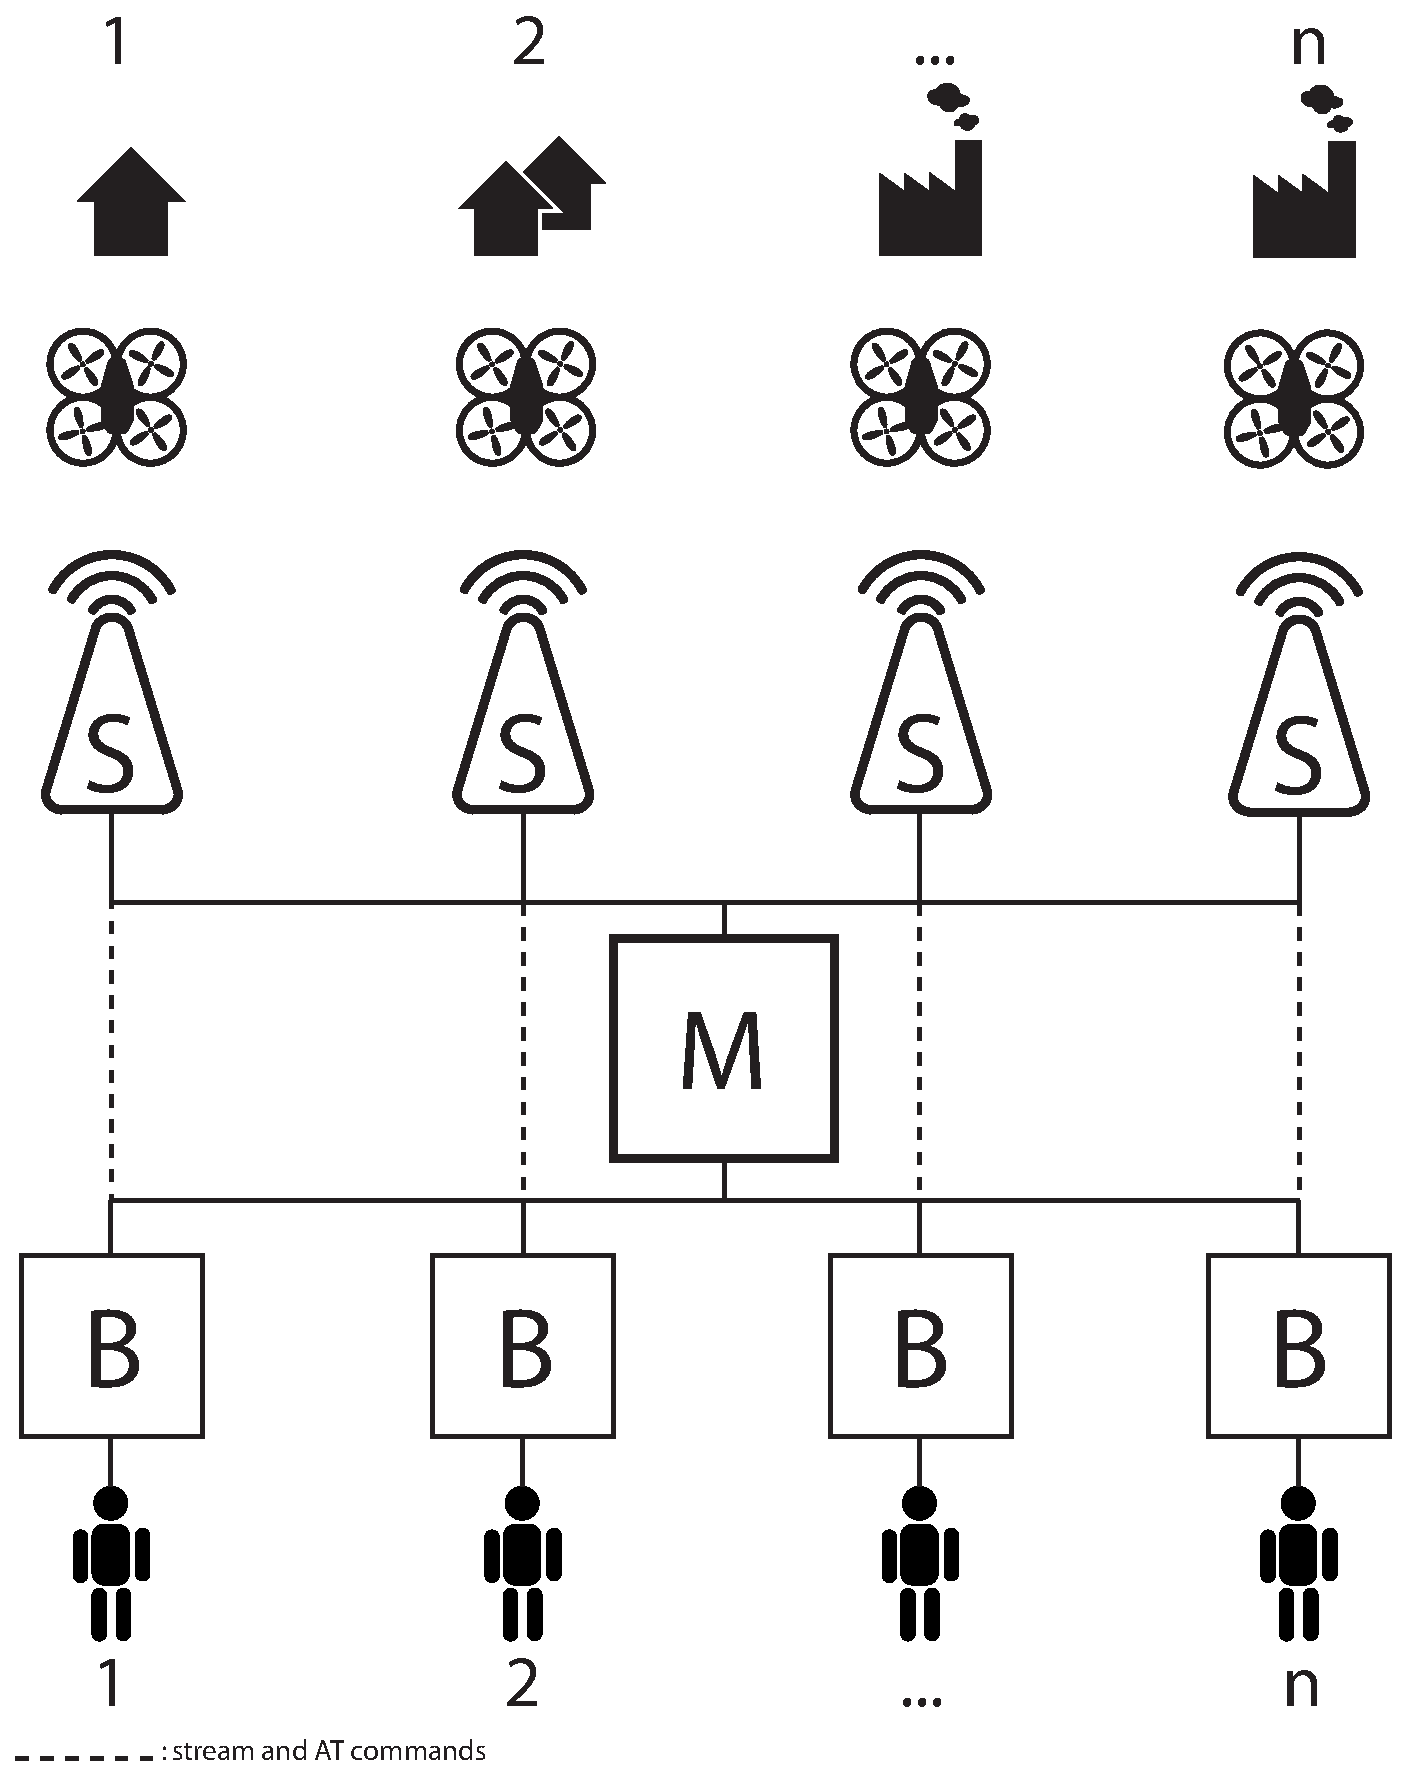
\includegraphics[width=\textwidth]{gfx/system_architecture.pdf}
    \caption{System architecture of \projectname{}}
    \label{fig:system_architecture}
\end{figure}

The system only uses one M. This is also the bottleneck of the system. If M crashes all S's and B's will have to wait for M to come back up.
One alternative could be running with more M's and in that way scale out.

There is always one S for each drone connected to the system. In this way the system is scaled out. This ensures that any S is not likely to become a bottleneck.
This was done because the drone uses wireless network which is short ranged and the drone is the host which means that the server needs one wireless connection for each drone it have to transmit to.
One alternative could be only running with one S and just scale it up. The problem with this is the server will need a wireless connection for each drone it have to control and it have to be in range.

Daemons is a background process on a Linux system.
Daemons is used when it is needed that a process is running at all times. In \projectname{} there are both the session key system which both resides on M and S and a policy file system for Adobe Flash on S. Both of these processes needs to be running at all times for the user to interact with the drone on S.

\fixme{Alternatives?}